We're going to present the first draft of the scheduling we would follow to develop this software. We tried to be as responding as possibile in the scheduling of what we have really done, that is RASD and DD development. For what concerns the successive phases, as we have never approached such a complex software, we made a rough estimation of the time each activity would take. As we gain experience along the real development, we could provide more precise estimation. We followed an overall waterfall approach.\\
We splitted images to enhance readibility, presenting the scheduling of each macro-activity.\\

\begin{figure}
\vspace*{-4cm}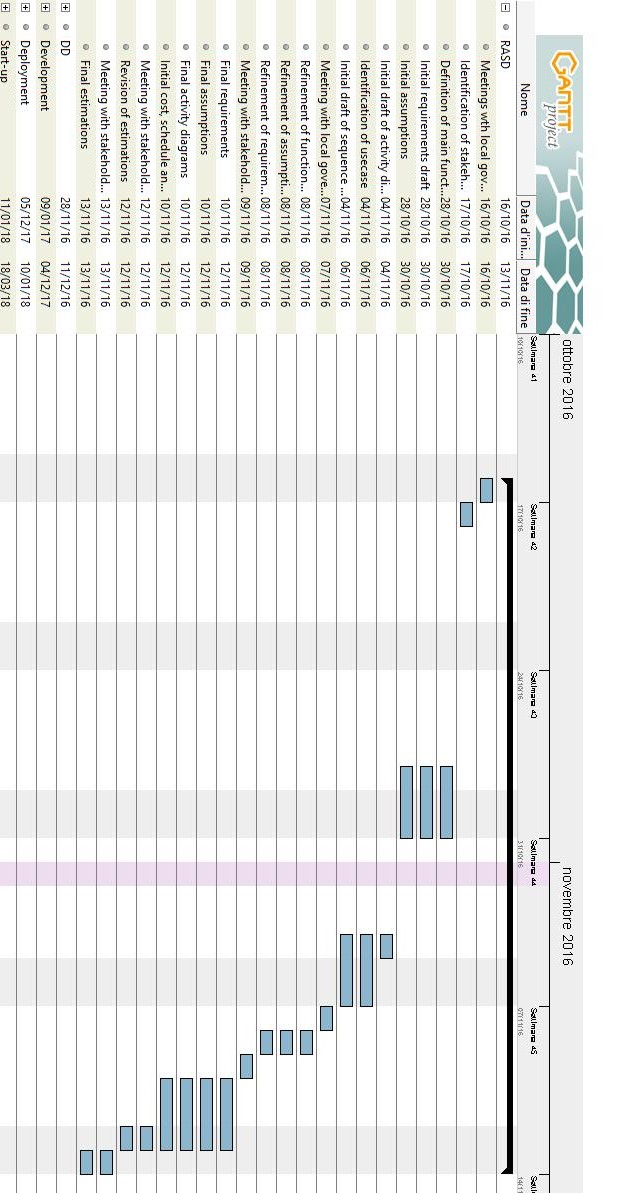
\includegraphics[scale=0.7]{Gantt_RASD}
\end{figure}
\begin{figure}
\vspace*{-4cm}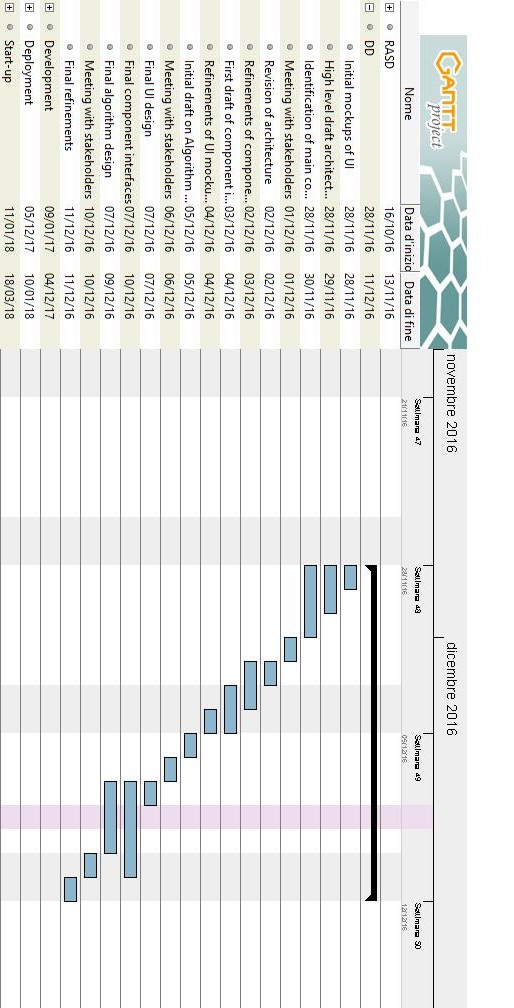
\includegraphics[scale=0.7]{Gantt_DD}
\end{figure}
\begin{figure}
\vspace*{-4cm}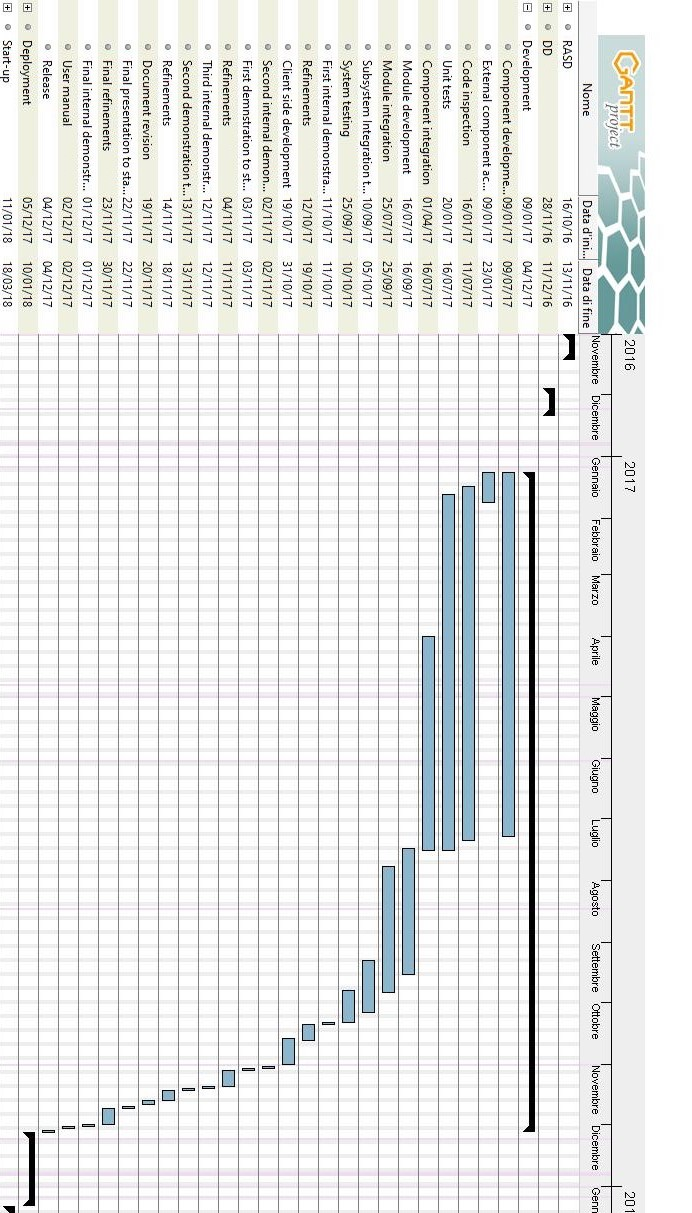
\includegraphics[scale=0.7]{Gantt_Development}
\end{figure}
\begin{figure}
\hspace*{+4cm}\vspace{-3.5cm}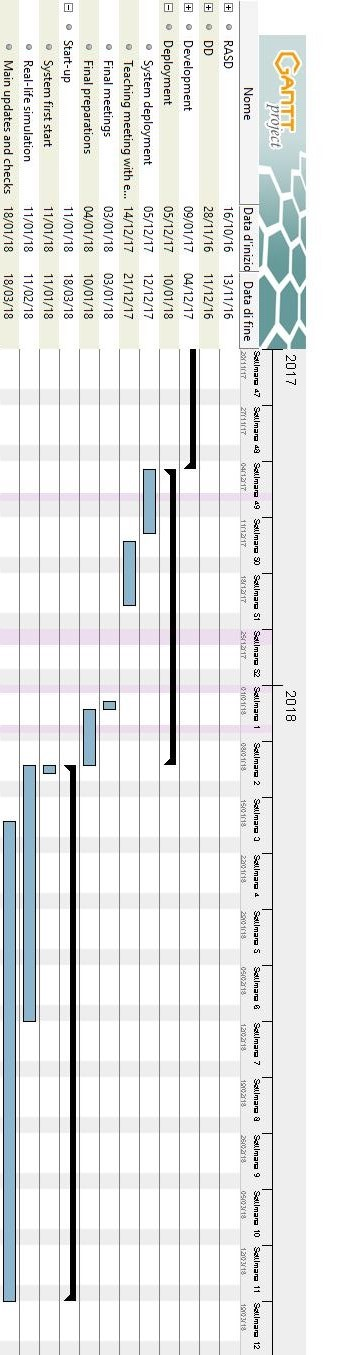
\includegraphics[scale=0.6]{Gantt_Deployment_Startup}
\end{figure}